\documentclass[12pt]{scrartcl}

\usepackage{graphicx}
\usepackage{geometry}
\usepackage[utf8]{inputenc}

\geometry{a4paper,left=20mm,right=20mm,top=10mm,bottom=20mm}
\setlength\parindent{0mm}

\title{Robotikpraktikum (FP) Webcam SS 2014}
\date{\vspace{-10ex}}

\begin{document}
\maketitle

\begin{figure}[h]
	\centering
	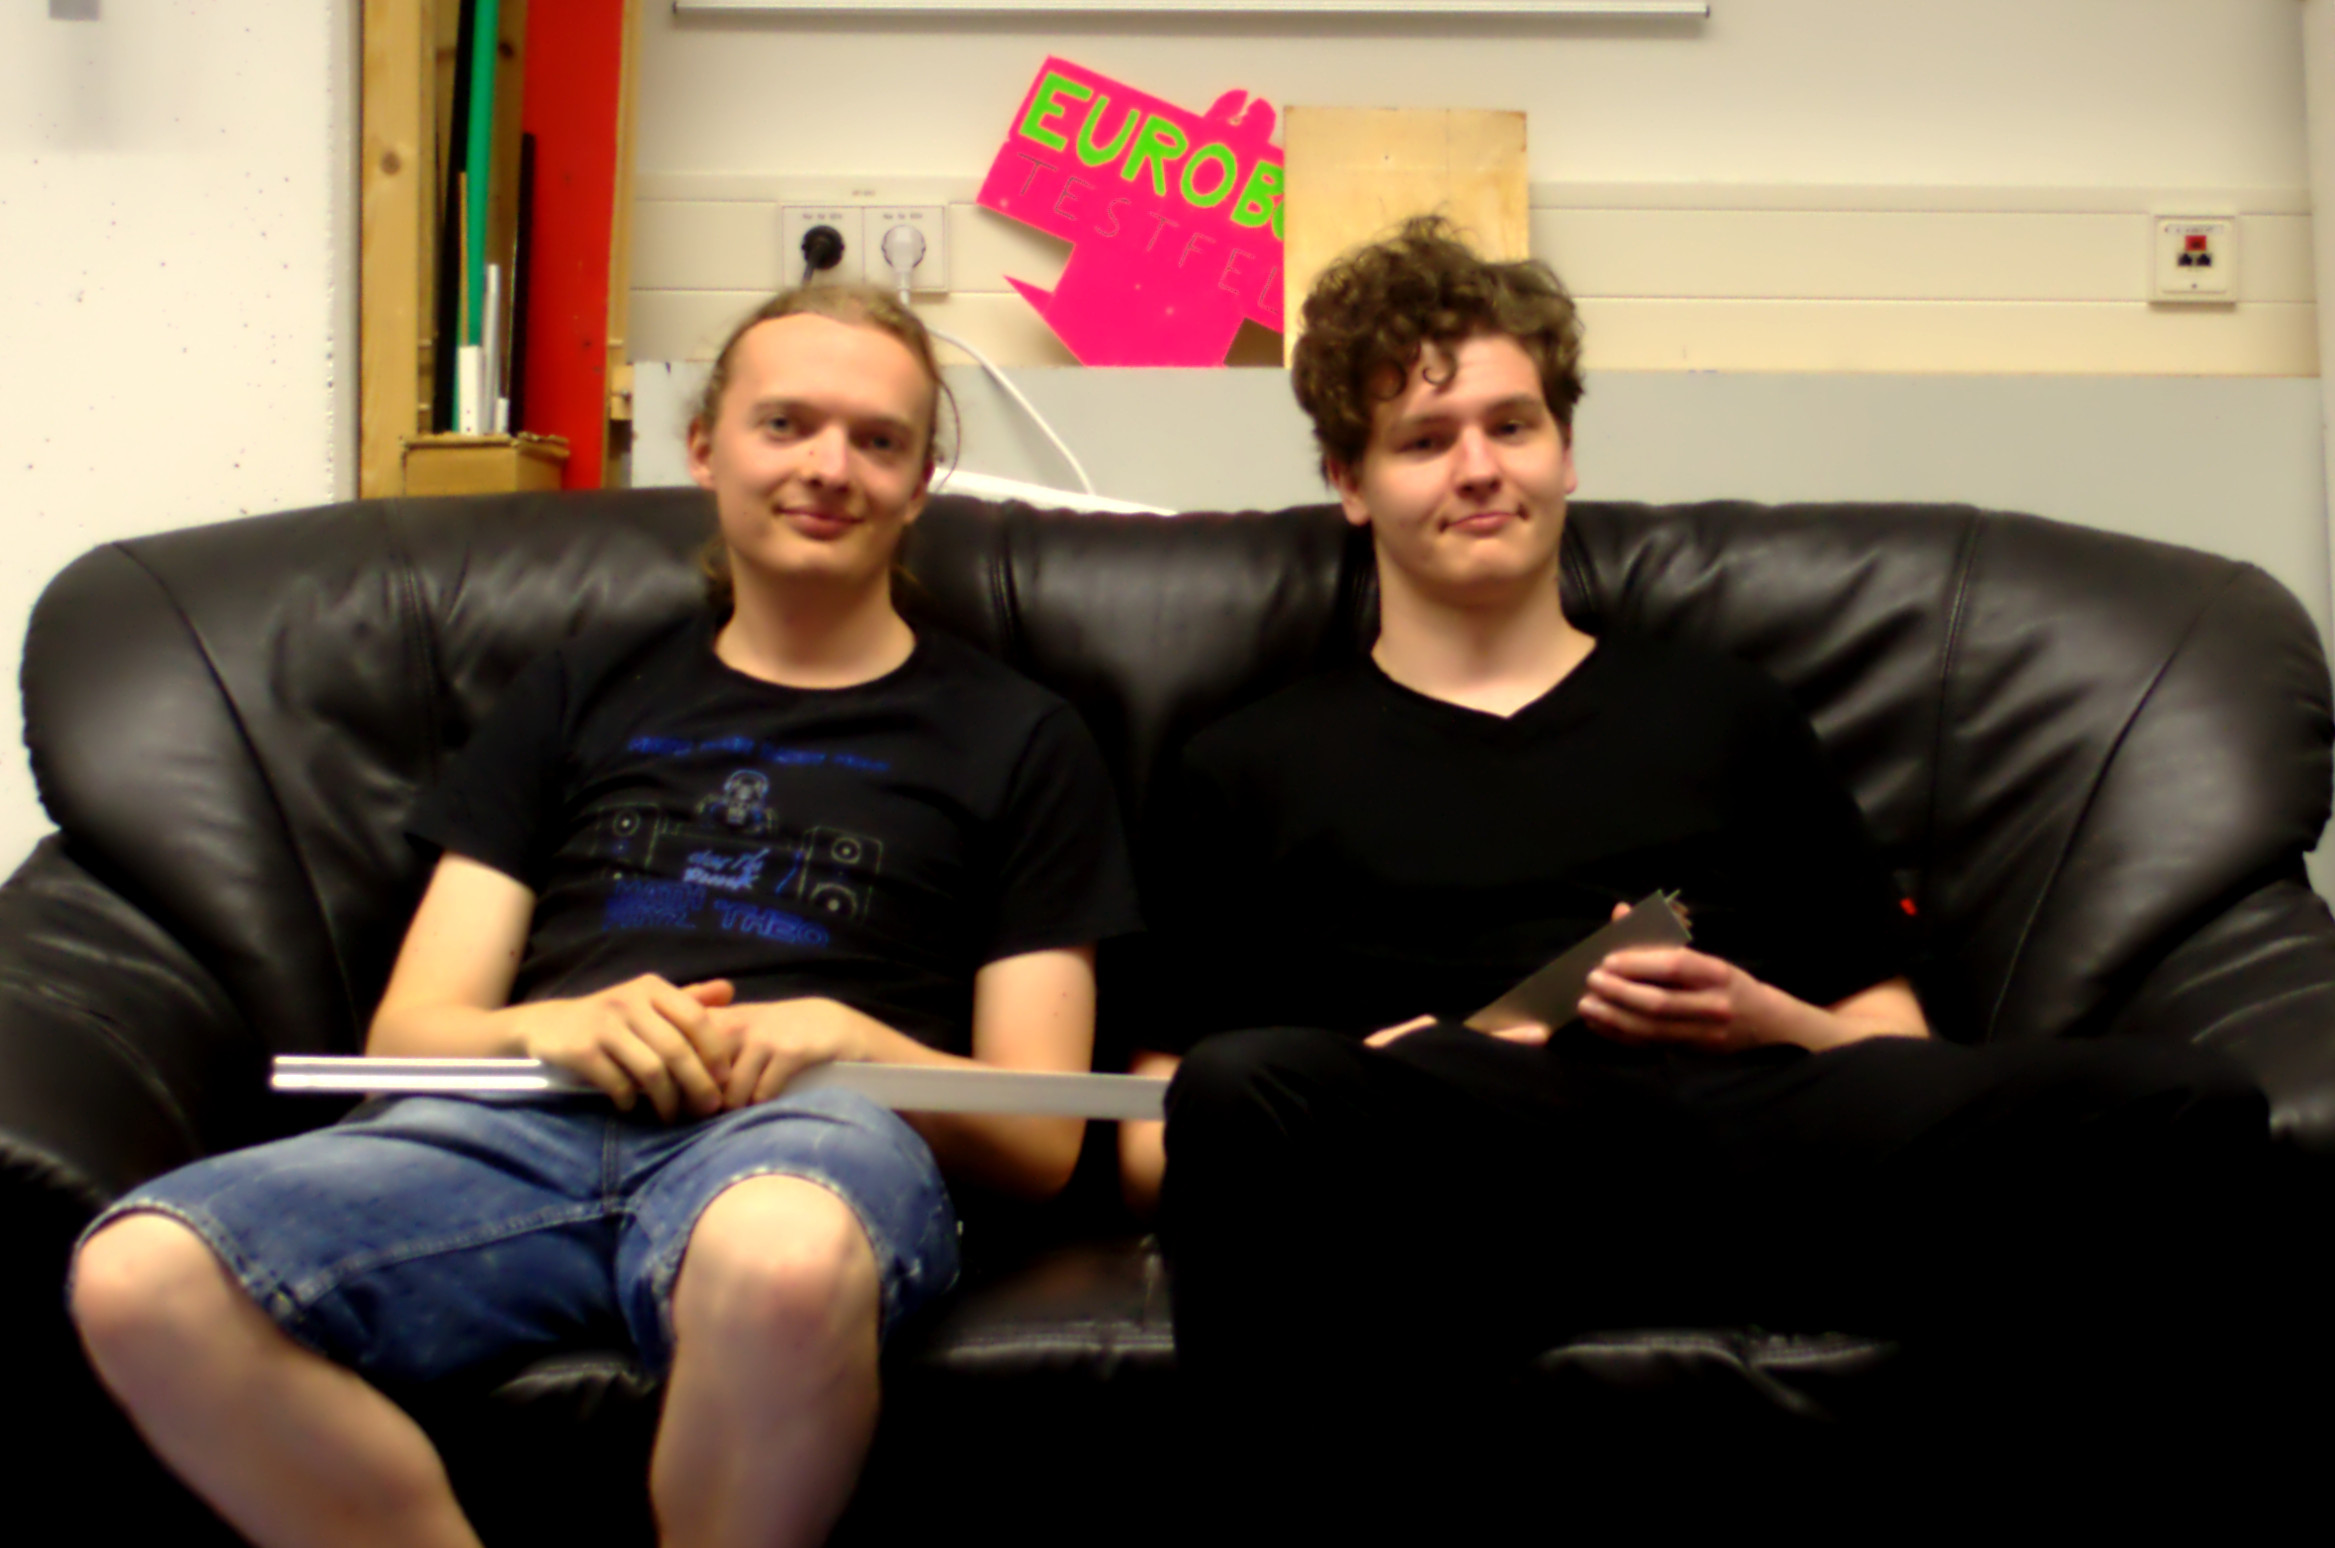
\includegraphics[width=1\textwidth]{steckbrief.jpg}
\end{figure}

\begin{tabular}{l l l}
	\textbf{Praktikanten:}	& Philip Bell,			& 6. Semester B.Sc. Mathematik\\
							& Johannes Visintini,	& 6. Semester B.Sc. Angewandte Informatik\\
	\textbf{Betreuer}: 		& Markus Kurz 			& \\
	\textbf{Supervisor}: 	& Thomas Klöpfer		&
\end{tabular}
\vspace{1.5em}

Ziel unseres Praktikums ist es, eine Webcam mit einem Raspberry Pi ansteuerbar
zu machen. Dazu sollen wir eine Webschnittstelle entwickeln, über diese die
Webcam (aus der Ferne) gesteuert werden soll. Weiterhin umfasst das Praktikum
den Bau einer Befestigung für die Webcam und ihre Steuereinrichtungen.

\section*{Milestones}
\begin{tabular}{l l}
	\textbf{Ende Juni:}			& Raspberry Pi fertig eingerichtet\\
								& Funktionsfähigkeit aller Komponenten getestet (Einarbeitungsphase)\\
	\textbf{Ende Juli:}			& Befestigung fertig gestellt\\
	\textbf{Mitte August:}		& Steuersoftware fertig gestellt\\
	\textbf{Ende August:}		& Webschnittstelle fertig gestellt\\
	\textbf{Mitte September:}	& Präsentation des Praktikums und Dokumentation fertig gestellt
\end{tabular}



\end{document}
